\documentclass[article,nojss]{jss}

\usepackage{listings}
\usepackage{hyperref}

\DeclareGraphicsExtensions{.pdf,.eps}
\newcommand{\fct}[1]{{\code{#1()}}}
\newcommand{\class}[1]{{`\code{#1}'}}


\author{Marco Smolla \And Bart Kranstauber}
\Plainauthor{Marco Smolla, Bart Kranstauber}

\title{An introduction to the 'move' package}
\Plaintitle{Using the move package}

\Keywords{animal track, time series, utilization density, gps}

\Abstract{
  The move package provides a series of functions to import, visualize and analyze animal movement related data in an object oriented way. The introduced classes allow to store data that are related to an individual in one object, such as coordinates and timestamps, name, species, age, sex, study site and so on. This makes working with multiple animals, or multiple seasons much easier. Furthermore, the package includes functions to calculate home ranges (Minimum Convex Polygon Bootstrap) and utilization distributions, UDs. The latter one uses the Dynamic Brownian Bridge Movement Model to calculate animal UDs.\\
}

\Address{
  Marco Smolla\\
  Max-Planck-Institute for Ornithology, Radolfzell, Germany\\
  E-mail: \email{msmolla@orn.mpg.de}\\

  Bart Kranstauber\\
  Max-Planck-Institute for Ornithology, Radolfzell, Germany\\
  E-mail: \email{kranstauber@orn.mpg.de}\\
}

\usepackage{Sweave}
\begin{document}
\input{move-concordance}


%\VignetteIndexEntry{How to use the move package}
%\VignetteDepends{sp, raster, rgdal, methods, geosphere}
%\VignetteKeywords{GPS, time series, track}
%\VignettePackage{move}


\section*{Introduction}
The amount of recorded animal movement data is increasing. The data offer information about land-use, distribution, interactions between the environment and much more. The enormous amount of data needs to be analyzed with mathematical algorithms. The programming language R, developed by the R Development Core Team, offers an easy to learn environment to do statistical analyzes. It even supports object oriented programming. The package we present here offers additional functions that are especially made to analyze animal movement data. \\
Movement data that are associated with individual animals or a group of animals can be imported into R and stored as a single object. These objects can include all kind of information. The minimum requirement however are timestamps, coordinates, and an unique ID per animal. Further attributes of the objects can be sensor types, body size, sex, weight, and so on. \\
A lot of data sets are available on a database called Movebank (\url{www.movebank.org}). If a user has the permission to see a data set, he can download it as a csv (comma separated values) file. Files from Movebank can be directly imported into R. \\
A more recent update of the Move package added a web-interface. Now, it is possible to directly download whole data-sets from within R. The only requirement is an account on Movebank and the rights to see the data (see the "browsing Movebank" vignette for more information). \\
Besides importing data from Movebank it is also possible to use own data-sets as long as they meet the minimum requirements of timestamps, coordinates and animal IDs. \\
A series of functions allows to plot, summarize and analyze the movement data. Individual \class{Move} objects can be stacked to a MoveStack object which includes a series of animals and the additional data that are associated with them. This allows to operate on many animals at the same time. \\
A new feature, called burst, allows to subset track information. This can be interesting for example if a track should be analyzed depending on specific behaviors (migratory, non-migratory, resting behavior). \\
One of the main features of the move package is the calculation of the Utilization Distribution (UD), a measure to estimate the home range of an animal. In this version of the package we use the Dynamic Brownian Bridge Movement Model (DBBMM) to calculate the UD. The UD can be calculated for individuals or for a stack of individuals. This results in the object types \class{DBBMM} or \class{DBBMMStack}. These objects store all information that are needed to visualize the UD, like the raster it was calculated for, and the values per raster cell.\\
The following sections introduce the different functions we implemented for the \class{Move}, \class{MoveStack}, \class{DBBMM}, and \class{DBBMMStack} objects. We demonstrate how functions can be used to import, analyze and visualize animal movement data. The aim of this vignette is to enable all users unfamiliar with the package to handle all basic functions.



%%%%%%%%%%%%%%%%%%%%%%%%%%%%%%%%%%%%%%%%%%%%%%%%%%%%%%%
\section{Data import}
The import of data into R can happen on two ways. Either by importing data files with a csv extension (using the \fct{move} function) or by using the web interface of the move package (using the \fct{getMovebankData} function). The web interface allows to access and download data sets from Movebank. 

\subsection{Import of Movebank data}
Files from Movebank (\url{www.movebank.org}) can be imported with \texttt{move(x="path")}, where "path" is character string which locates the file on the hard-drive. It may look like: \\ \\ \texttt{> data <- move(x="/User/Documents/test.csv")}. \\ \\
The following line imports the "leroy.csv" filet that is part of the move package.

\begin{Schunk}
\begin{Sinput}
> leroy <- move(system.file("extdata","leroy.csv",package="move"))
\end{Sinput}
\end{Schunk}

\subsection{Import of non-Movebank data}
If data sets are not published on Movebank but stored on the hard drive they can be imported with the same \fct{move} function. Because the column names may differ from the Movebank standard, it is necessary to indicate the timestamp and coordinates columns and the projection method of the coordinates (e.g. longitude-latitude), and the data-frame that includes all the imported data. The standard \fct{move} method also allows to directly enter the used sensor type and the animal name. \\
Import of a non-Movebank csv file that is attached to this package:

\begin{Schunk}
\begin{Sinput}
> data <- read.csv(system.file("extdata","ricky.csv",package="move"))
> ricky <- move(x=data$location.long, y=data$location.lat, time=as.POSIXct(data$timestamp, 
+             format="%Y-%m-%d %H:%M:%OS", tz="UTC"), proj=CRS("+proj=longlat"), 
+             data=data, animal=data$individual.local.identifier, sensor=data$sensor)
> ricky 
\end{Sinput}
\begin{Soutput}
class       : Move 
nfeatures   : 8961 
extent      : -74.00481, -73.84202, 42.80671, 42.89606  (xmin, xmax, ymin, ymax)
coord. ref. : +proj=longlat +ellps=WGS84 
nvariables  : 19
variables   : event.id, eobs.battery.voltage, eobs.fix.battery.voltage, eobs.horizontal.accuracy.estimate, eobs.key.bin.checksum, eobs.speed.accuracy.estimate, eobs.start.timestamp, eobs.temperature, eobs.used.time.to.get.fix, ground.speed, heading, height.above.ellipsoid, manually.marked.outlier, visible, individual.local.identifier, ... 
min values  : 44295482, 3449, 3081,  2.05,     524362,  0.22, 2010-02-09 17:00:00.000,   0,   3,  0.00,   0.00,    0.0, , false, Ricky.T, ... 
max values  : 44529025, 3740, 3559, 95.23, 4294919150, 48.67, 2010-03-31 17:30:02.000, -12, 120, 43.12, 359.79, 9318.3, true, true, Ricky.T, ... 
timestamps  : 2010-02-09 17:01:23...2010-03-31 17:31:26 Time difference of 50 days  (start...end, duration) 
sensors     : gps 
indiv. data : behavioural.classification, eobs.status, eobs.type.of.fix, sensor.type, individual.taxon.canonical.name, tag.local.identifier, study.name, utm.zone, study.timezone 
missed fixes : 1888 
date created: 2012-09-07 16:18:58 
\end{Soutput}
\end{Schunk}

Entering the object name calls the \fct{show} function of \class{Move} objects. This function provides an overview of the object. It returns the object class (\class{Move}), the animal ID (ricky), number of coordinates (8961), the extent of the coordinates, the coordinates reference system (or projection, here longitude-latitude), the number of columns of the imported data.frame and the names of the columns of the data.frame, as well es the first and last timestamp and the duration of the observation.The \fct{show} works in a similar way for all other object types.\\


\subsection{Handling multiple animals}
If the data-set includes more than one animal, it is necessary to indicate the column with the animal IDs. The \fct{move} automatically creates a stack of Move objects called \class{MoveStack}. \\
Sometimes it is desirable to work with stacked Move objects. The most functions of the Move package are capable to work with stacks. Stacks are either created when csv files with multiple animal IDs are imported, or when a \class(list) of \class(Move) objects is passed on to the staking function \fct{moveStack}.

\begin{Schunk}
\begin{Sinput}
> list <- list(leroy, ricky)
> stack <- moveStack(list)
> stack
\end{Sinput}
\begin{Soutput}
class       : MoveStack 
nfeatures   : 9880 
extent      : -74.00481, -73.84202, 42.70898, 42.89606  (xmin, xmax, ymin, ymax)
coord. ref. : +proj=longlat +ellps=WGS84 +datum=WGS84 +towgs84=0,0,0 
nvariables  : 19
variables   : eobs.battery.voltage, eobs.horizontal.accuracy.estimate, eobs.key.bin.checksum, eobs.speed.accuracy.estimate, eobs.start.timestamp, eobs.temperature, eobs.used.time.to.get.fix, ground.speed, heading, height.above.ellipsoid, individual.local.identifier, utm.easting, utm.northing, study.local.timestamp, sensor, ... 
min values  : 3449,  2.05,     524362,  0.22, 2009-02-11 12:14:59.000,   0,   3,  0.00,   0.00,    0.0, Leroy, 581253.3, 4729143, 2009-02-11 07:16:45, gps, ... 
max values  : 3740, 97.02, 4294919150, 48.67, 2010-03-31 17:30:02.000, -12, 120, 43.12, 359.79, 9318.3, Ricky.T, 594680.9, 4749753, 2010-03-31 13:31:26, gps, ... 
timestamps  : 2009-02-11 13:16:45...2010-03-31 19:31:26 Time difference of 413 days  (start...end, duration) 
sensors     : gps 
indiv. data : eobs.fix.battery.voltage, eobs.status, eobs.type.of.fix, manually.marked.outlier, visible, individual.taxon.canonical.name, tag.local.identifier, study.name, utm.zone, study.timezone, behavioural.classification, sensor.type 
individuals : Leroy, Ricky.T 
date created: 2012-09-07 16:18:58 
\end{Soutput}
\end{Schunk}

The show function works also for the stack object. It combines the information of all objects that are stored in the \class{MoveStack}. \\
It is also possible to break down a \class{MoveStack} into single \class{Move} objects using the \fct{split} function. It returns a list of all \class{Move} objects.


\begin{Schunk}
\begin{Sinput}
> unstacked <- split(stack)
> #use show(unstacked) to see all objects of unstacked
\end{Sinput}
\end{Schunk}

\subsection{Import of Movebank data-sets using the web-interface}
The Move package includes a bunch of functions to access the Movebank database. With \fct{getMovebankData} whole data sets can be downloaded and stored as a \class{Move} or \class{MoveStack} object (we can \textbf{not} offer a \textbf{working example} in this vignette due to fact that Movebank does not allow dummy accounts). You can use the function as follows: \\ \\ \texttt{> bobby <- getMovebankData(study="BCI Ocelot", animalName="Bobby", login=abc)} \\ \\ With this command the data associated with the animal ID "Bobby" from the study "BCI Ocelot" is stored in a \class{Move} object (because it is only one animal) called \texttt{bobby}. \\ The following command will download the full study: \\ \\ \texttt{> ocelot <- getMovebankData(study="BCI Ocelot", login=abc)} \\ \\ This function will create a \class{MoveStack} object. Note, it is necessary to provide a login object to access the Movebank database. More information about the Movebank browsing functions are in the additional vignette "browsing Movebank".


\newpage
%%%%%%%%%%%%%%%%%%%%%%%%%%%%%%%%%%%%%%%%%%%%%%%%%%%%%%%
\section{Visualizing and analyzing Move objects}
In the previous chapter we presented the \fct{moveStack} and \fct{split} functions to stack and unstack \class{Move} objects. In this chapter we present further functions to work with the two object types. 

\subsection{Show and summarize} 
An important function to work with objects is the \fct{show} function. Depending on the implementation it gives an overview of the object one is working with. The function can either called by entering the name of the object directly, or by calling the function with the object:

\begin{Schunk}
\begin{Sinput}
> show(leroy)
\end{Sinput}
\begin{Soutput}
class       : Move 
nfeatures   : 919 
extent      : -73.93067, -73.84366, 42.70898, 42.7687  (xmin, xmax, ymin, ymax)
coord. ref. : +proj=longlat +ellps=WGS84 +datum=WGS84 +towgs84=0,0,0 
nvariables  : 15
variables   : eobs.battery.voltage, eobs.horizontal.accuracy.estimate, eobs.key.bin.checksum, eobs.speed.accuracy.estimate, eobs.start.timestamp, eobs.temperature, eobs.used.time.to.get.fix, ground.speed, heading, height.above.ellipsoid, individual.local.identifier, utm.easting, utm.northing, study.local.timestamp, sensor 
min values  : 3596,  3.07,    3258904,  0.27, 2009-02-11 12:14:59.000, 13,   4,  0.01,   0.00,    3.3, Leroy, 587507.8, 4729143, 2009-02-11 07:16:45, gps 
max values  : 3666, 97.02, 4291715164, 33.04, 2009-03-04 09:15:01.000, 35, 119, 31.71, 359.79, -169.6, Leroy, 594679.4, 4735720, 2009-03-04 04:16:59, gps 
timestamps  : 2009-02-11 12:16:45...2009-03-04 09:16:59 Time difference of 21 days  (start...end, duration) 
sensors     : gps 
indiv. data : eobs.fix.battery.voltage, eobs.status, eobs.type.of.fix, manually.marked.outlier, visible, individual.taxon.canonical.name, tag.local.identifier, study.name, utm.zone, study.timezone 
missed fixes : 1071 
date created: 2012-09-07 16:18:58 
\end{Soutput}
\end{Schunk}

Both ways return the same information. This is for Move objects the class name, number of coordinates, the map extent, the coordinate reference system, number of additional variables, names of the additional variables and their minimum and maximum values, the sensor type, further data that are specific to the animal, the number of recordings that were skipped and the date of file creation. \\
The \fct{summary} can be used to summarize important information of \class{Move} or \class{MoveStack} objects. \fct{Summary} calls the function \fct{distance}, \fct{time}, \fct{speed}, and \fct{angle} and returns a summary of these values. 

\begin{Schunk}
\begin{Sinput}
> summary(ricky)
\end{Sinput}
\begin{Soutput}
$Ricky.T
  TravDist  MaxDist   MinDist FarthDist AverDist   SDDist   SEDist
1   409134 7758.682 0.1573102  10181.32 45.66227 159.2503 759.3597

$Ricky.T
        Duration  AverDur   SDDur  dupl multseason
1 1200.501 hours 482.3441 2638.43 FALSE       TRUE

$Ricky.T
  AverSpeed VarSpeed MaxSpeed
1 0.3290363 2.882038 100.7703

$Ricky.T
  AverAzimuth VarAzimuth SEAzimuth
1   -153.0871  0.9906407  16.37971
\end{Soutput}
\begin{Sinput}
> #summary(stack) ##works also for stacks
\end{Sinput}
\end{Schunk}

More information of the object do the following functions return: 
\fct{n.locs} returns the number of locations of an \class{Move} or \class{MoveStack} object
\begin{Schunk}
\begin{Sinput}
> n.locs(ricky)
\end{Sinput}
\begin{Soutput}
[1] 8961
\end{Soutput}
\end{Schunk}
\fct{time.lag} returns the time differences between successive coordinates from \class{Move} or \class{MoveStack} objects (the\texttt{units} argument determines the units of the data output, it is minutes by default)
\begin{Schunk}
\begin{Sinput}
> head(time.lag(leroy, units="mins"))
\end{Sinput}
\begin{Soutput}
[1] 14.88333 14.18330 14.45007 15.04998 14.90000 15.39998
\end{Soutput}
\end{Schunk}
\fct{timestamps} returns all time-stamps of an \class{Move} or \class{MoveStack} object
\begin{Schunk}
\begin{Sinput}
> head(timestamps(leroy))
\end{Sinput}
\begin{Soutput}
[1] "2009-02-11 12:16:45 UTC" "2009-02-11 12:31:38 UTC"
[3] "2009-02-11 12:45:48 UTC" "2009-02-11 13:00:16 UTC"
[5] "2009-02-11 13:15:19 UTC" "2009-02-11 13:30:13 UTC"
\end{Soutput}
\end{Schunk}



\subsection{Plot}
A simple plotting function is implemented both for \class{Move} and \class{MoveStack} objects. The \fct{plot} function uses arguments from the generic plot function to change plot properties. In the example below the arguments \texttt{col} (color), \texttt{lwd} (line width), \texttt{pch} (point character), and \texttt{xlab} and \texttt{ylab} (x and y labels) are used to adjust the graphs (see Figure. \ref{fig:one}). 

\begin{Schunk}
\begin{Sinput}
> par(mfcol=1:2)
> plot(leroy, type="o", col=3, lwd=2, pch=20, xlab="location_long", 
+      ylab="location_lat")
> plot(stack, col=c(6,5), lwd=2, xlab="location_long", ylab="location_lat")
\end{Sinput}
\end{Schunk}

\setkeys{Gin}{width=0.8\textwidth}

\begin{figure}
\begin{center}
\includegraphics{move-figTrack}
\end{center}
\caption{Using the \fct{plot} function to plot the track and its coordinates of a \class{Move} (left) and a \class{MoveStack} (right) object.}
\label{fig:one}
\end{figure}


\subsection{Google plot}
An interesting addition to plot the pure track is to plot the track on a map. The easiest way to use for example OpenStreetMap, Stamen Map, Cloudmade or Google Maps is to use the ggmap package, which is based on ggplot.\\
Note, that the function requires two further packages (\texttt{ggmap} and \texttt{mapproj}). The \fct{get\_map} function makes a call to the online data bases and retrieves a map which is defined by the bounding box (\texttt{bbox}). The source argument allows to choose between OpenStreetMap (\texttt{'osm'}), Stamen Maps (\texttt{'stamen'}), Clodumade (\texttt{'cloudmade'}) and Google Maps (\texttt{'google'}). The \fct{ggmap} function plots the map in a new graphics device and \texttt{geom\_path()} adds the track of the \class{Move} object (see Figure \ref{fig:google}).  

\begin{Schunk}
\begin{Sinput}
> require(ggmap) #these packages are necessecary to work with google maps
> require(mapproj)
> leroy_df <- as(leroy, "data.frame")
> m <- get_map(bbox(extent(leroy)*1.1), source="stamen", zoom=14)
> ggmap(m)+geom_path(data=leroy_df, aes(x=coords.x1, y=coords.x2))
\end{Sinput}
\end{Schunk}
\begin{figure}
\begin{center}
\includegraphics{move-figGoogle}
\end{center}
\caption{Plotting a track on a map using \fct{ggmap}.}
\label{fig:google}
\end{figure}



\subsection{Subset and transform objects}
Sometimes only a subset of all coordinates of an animal track is needed. With the subset function a section of all coordinates are returned as a new \class{Move} or \class{MoveStack} object. 

\begin{Schunk}
\begin{Sinput}
> ricky[1:25]
\end{Sinput}
\begin{Soutput}
class       : Move 
nfeatures   : 25 
extent      : -73.90426, -73.90235, 42.84125, 42.84189  (xmin, xmax, ymin, ymax)
coord. ref. : +proj=longlat +ellps=WGS84 
nvariables  : 19
variables   : event.id, eobs.battery.voltage, eobs.fix.battery.voltage, eobs.horizontal.accuracy.estimate, eobs.key.bin.checksum, eobs.speed.accuracy.estimate, eobs.start.timestamp, eobs.temperature, eobs.used.time.to.get.fix, ground.speed, heading, height.above.ellipsoid, manually.marked.outlier, visible, individual.local.identifier, ... 
min values  : 44528398, 3518, 3388,  4.86,   33124537,  1.64, 2010-02-09 17:00:00.000,   1,   7,  0.07,   0.66,  39.3, , true, Ricky.T, ... 
max values  : 44528427, 3662, 3493, 39.42, 4285600836, 18.80, 2010-02-09 20:58:01.000, -12, 118, 14.71, 359.14, 128.5, , true, Ricky.T, ... 
timestamps  : 2010-02-09 17:01:23...2010-02-09 20:58:51 Time difference of 4 hours  (start...end, duration) 
sensors     : gps 
indiv. data : behavioural.classification, eobs.status, eobs.type.of.fix, sensor.type, individual.taxon.canonical.name, tag.local.identifier, study.name, utm.zone, study.timezone 
missed fixes : 1888 
date created: 2012-09-07 16:18:58 
\end{Soutput}
\begin{Sinput}
> stack[800:1100] #see the names of both animals in second last row
\end{Sinput}
\begin{Soutput}
class       : MoveStack 
nfeatures   : 301 
extent      : -73.91325, -73.86532, 42.72992, 42.84189  (xmin, xmax, ymin, ymax)
coord. ref. : +proj=longlat +ellps=WGS84 +datum=WGS84 +towgs84=0,0,0 
nvariables  : 19
variables   : eobs.battery.voltage, eobs.horizontal.accuracy.estimate, eobs.key.bin.checksum, eobs.speed.accuracy.estimate, eobs.start.timestamp, eobs.temperature, eobs.used.time.to.get.fix, ground.speed, heading, height.above.ellipsoid, individual.local.identifier, utm.easting, utm.northing, study.local.timestamp, sensor, ... 
min values  : 3500,  3.07,   33124537,  0.58, 2009-03-01 11:45:01.000,   0,   4,  0.02,   0.00,    2.3, Leroy, 588917.9, 4731448, 2009-03-01 06:45:50, gps, ... 
max values  : 3725, 67.33, 4285600836, 27.96, 2010-02-11 05:39:59.000, -12, 120, 31.71, 359.14, -127.7, Ricky.T, 592890.4, 4743839, 2010-02-11 00:40:38, gps, ... 
timestamps  : 2009-03-01 12:45:50...2010-02-11 06:40:38 Time difference of 347 days  (start...end, duration) 
sensors     : gps 
indiv. data : eobs.fix.battery.voltage, eobs.status, eobs.type.of.fix, manually.marked.outlier, visible, individual.taxon.canonical.name, tag.local.identifier, study.name, utm.zone, study.timezone, behavioural.classification, sensor.type 
individuals : Leroy, Ricky.T 
date created: 2012-09-07 16:18:58 
\end{Soutput}
\end{Schunk}

If it is necessary to directly interact with different data of the same object it can be advantageous to work with a data.frame. The \fct{as} function can transform a \class{Move} or \class{MoveStack} to a data.frame:

\begin{Schunk}
\begin{Sinput}
> head(as(leroy, "data.frame"))
\end{Sinput}
\begin{Soutput}
   eobs.battery.voltage eobs.horizontal.accuracy.estimate eobs.key.bin.checksum
45                 3615                             14.85            2992317972
46                 3623                              5.38            1723246055
47                 3627                              5.38            1910450098
48                 3632                              6.40            2286746099
49                 3642                              7.68            3797866101
50                 3647                              8.70            3956003832
   eobs.speed.accuracy.estimate    eobs.start.timestamp eobs.temperature
45                         5.65 2009-02-11 12:14:59.000               20
46                         4.69 2009-02-11 12:30:01.000               26
47                         4.19 2009-02-11 12:45:01.000               24
48                         5.97 2009-02-11 13:00:02.000               24
49                         6.34 2009-02-11 13:15:01.000               25
50                         6.15 2009-02-11 13:30:01.000               23
   eobs.used.time.to.get.fix ground.speed heading height.above.ellipsoid
45                       106         2.10  125.17                   79.3
46                        97         0.51    3.28                   94.2
47                        47         0.16   91.10                   82.5
48                        14         0.23  335.54                  153.7
49                        18         0.48  359.79                   73.7
50                        12         0.17   29.49                   71.2
   individual.local.identifier utm.easting utm.northing study.local.timestamp
45                       Leroy    590130.0      4732942   2009-02-11 07:16:45
46                       Leroy    590136.3      4732940   2009-02-11 07:31:38
47                       Leroy    590138.5      4732935   2009-02-11 07:45:48
48                       Leroy    590144.0      4732947   2009-02-11 08:00:16
49                       Leroy    590137.0      4732940   2009-02-11 08:15:19
50                       Leroy    590126.0      4732936   2009-02-11 08:30:13
   sensor coords.x1 coords.x2 sensor.1          timestamps
45    gps -73.89880  42.74370      gps 2009-02-11 12:16:45
46    gps -73.89872  42.74369      gps 2009-02-11 12:31:38
47    gps -73.89869  42.74364      gps 2009-02-11 12:45:48
48    gps -73.89862  42.74374      gps 2009-02-11 13:00:16
49    gps -73.89871  42.74368      gps 2009-02-11 13:15:19
50    gps -73.89885  42.74365      gps 2009-02-11 13:30:13
\end{Soutput}
\end{Schunk}

For technical reasons the coordinates of the Move object must be in \texttt{aeqd} projection, which stands for Azimuthal Equidistant. To check the projection of your coordinates you can use the \fct{proj4string} method. If your data are not in the right projection, use the following command to change it. 

\begin{Schunk}
\begin{Sinput}
> proj4string(leroy)
\end{Sinput}
\begin{Soutput}
[1] " +proj=longlat +ellps=WGS84 +datum=WGS84 +towgs84=0,0,0"
\end{Soutput}
\begin{Sinput}
> leroy_t <- spTransform(x=leroy, CRSobj="+proj=aeqd", center=TRUE)  
> proj4string(leroy_t)
\end{Sinput}
\begin{Soutput}
[1] " +proj=aeqd +ellps=WGS84 +lon_0=-73.8871629 +lat_0=42.73884025"
\end{Soutput}
\end{Schunk}

The data are now in the right projection and the coordinate system is now centered to the center of the track. 


\subsection{Bursting tracks}
It can be interesting to compare different parts of the track with each other. For example: how do data points differ between winter and summer, or between behaviors like migrating, non-migrating, resting? To indicate which point of the data set belongs to which category a track is 'bursted'. This means, that an additional column is introduced to the data set that is associated with a category and all other track information. \\
A track is bursted by supplying a vector with the length of the number of coordinates. The vector is than used as a factor to be associated with the \class{Move} object. The returned object belongs to the class \class{MoveBurst}. 

\begin{Schunk}
\begin{Sinput}
> behavior <- c(rep(1:8,each=111), rep(1, 30))
> leroy_b <- burst(x=leroy, f=behavior)
> class(leroy_b)
\end{Sinput}
\begin{Soutput}
[1] "MoveBurst"
attr(,"package")
[1] "move"
\end{Soutput}
\end{Schunk}

Bursted tracks can be plotted with the basic \fct{plot} and the more complex \fct{plotBursts} function. Both functions use colors to indicate to which burstID a segment belongs. \\
The \fct{plot} function simply plots the different segments as colored lines. (see in the code example also a way to plot points instead of colored line segments) \\
The \fct{plotBursts} plots a circle for every segment right at the midpoint of the segment. The circles have a size that that is calculated with an extra size function. By default it is the relative time of the segment compared to the whole track. It is possible to calculate the size with a different function using the \texttt{sizeFun} argument of the function. (Figure \ref{fig:burst})

\begin{figure}
\begin{center}
\begin{Schunk}
\begin{Sinput}
> par(mfrow=c(2,2))
> plot(leroy_b, type="l", lwd=2)
> plot(midPoint(coordinates(leroy_b)[-n.locs(leroy_b), ], coordinates(leroy_b)[-1, ]), 
+      col=leroy_b@burstId, pch=20)
> plotBursts(leroy_b, breaks=3, add=FALSE, pch=19)
\end{Sinput}
\end{Schunk}
\includegraphics{move-figburst}
\end{center}
\caption{Plotting the track and adding the burst information as colored lines, poins or circles (the color corresponds to the brustID; the size of the circles represents in three steps the realtive amount of time per segment)}
\label{fig:burst}
\end{figure}

%%%%%%%%%%%%%%%%%%%%%%%%%%%%%%%%%%%%%%%%%%%%%%%%%%%%%%%
\newpage
\section{Dynamic Brownian Bridge Movement Model}
To calculate the utilization distribution (UD) with the dynamic Brownian Bridge Movement Model use the \fct{brownian.bridge.dyn} function. You need to specify the Move object from which you want to calculate the UD, the location error of your localization method (in map units), the raster options, and the extension of the raster. \\
You can either set the number of the raster cells along the longest dimension of your map by setting a numeric value for the \texttt{dimSize} argument, or - if you know the extent of your map - you can set the size of the raster cells with a numeric value for the \texttt{raster} argument (you can only set one of them). \\
When the \fct{brownian.bridge.dyn} function issues the warning, the extent of your raster is too small, that is that a large part of the UD is at the borders of the raster. You can change the extent of the raster by setting the \texttt{ext} argument. If you want to extend the raster in all four directions equally choose one number. Use a vector of two numbers to extend the x and the y dimension differently, or even a vector with four numbers to extend differently in all four directions.

\begin{Schunk}
\begin{Sinput}
> r <- spTransform(ricky[1:500,], center=T)
> ricky_dbbmm <- brownian.bridge.dyn(r, dimSize=150, location.error=23, ext=.3, time.step=60)
\end{Sinput}
\begin{Soutput}
[1] "Computational size: 2.4e+06"
\end{Soutput}
\end{Schunk}

Running the \fct{brownian.bridge.dyn} creates an object of the \class{DBBMM} class, which among others stores the raster of the map with the values from the UD. You can also run the function with a \class{MoveStack}. The returned object will then be a \class{DBBMMStack}.\\
The \class{DBBMM} and \class{DBBMMStack} objects can be summarized with the \fct{show} function (using the show function directly or by using the object name):

\begin{Schunk}
\begin{Sinput}
> ricky_dbbmm
\end{Sinput}
\begin{Soutput}
class       : DBBMM 
dimensions  : 122, 150, 18300  (nrow, ncol, ncell)
resolution  : 31.03099, 31.03099  (x, y)
extent      : -2327.14, 2327.509, -1892.768, 1893.013  (xmin, xmax, ymin, ymax)
coord. ref. : +proj=aeqd +ellps=WGS84 +lon_0=-73.8864686 +lat_0=42.83130625 
data source : in memory
names       : layer 
values      : 9.506822e-33, 0.02458818  (min, max)
\end{Soutput}
\begin{Sinput}
> raster(ricky_dbbmm)
\end{Sinput}
\begin{Soutput}
class       : RasterLayer 
dimensions  : 122, 150, 18300  (nrow, ncol, ncell)
resolution  : 31.03099, 31.03099  (x, y)
extent      : -2327.14, 2327.509, -1892.768, 1893.013  (xmin, xmax, ymin, ymax)
coord. ref. : +proj=aeqd +ellps=WGS84 +lon_0=-73.8864686 +lat_0=42.83130625 
\end{Soutput}
\end{Schunk}

The second method (\fct{raster}) returns all important information of the raster that is stored in the \class{DBBMM} object. \\
If only certain objects of a \class{DBBMMStack} are needed, the stack can be splitted into a \class{list} of \class{DBBMM} objects using the \fct{split} function.

\subsection{Plotting UDs}
\class{DBBMM} objects can be plotted with the \fct{plot} function. It produces a fixed cell size ratio graphic from the raster (see Figure \ref{fig:two}). A second function - \fct{image} - produces a variable cell size ratio graphic (not prone to distortions after resizing the graphics window) from the raster. \\


%\setkeys{Gin}{width=0.8\textwidth}

\begin{figure}
\begin{center}
\begin{Schunk}
\begin{Sinput}
> par(mfrow=c(1,2))
> plot(ricky_dbbmm, xlab="location_long", ylab="location_lat")
> plot(ricky_dbbmm, xlab="location_long", ylab="location_lat")
> lines(spTransform(ricky[1:500,], center=TRUE), col=3, lwd=2)
> #plot(ricky_dbbmm, xlab="location_long", ylab="location_lat")
> #points(spTransform(ricky[1:500, ], center=TRUE), col=8)
\end{Sinput}
\end{Schunk}
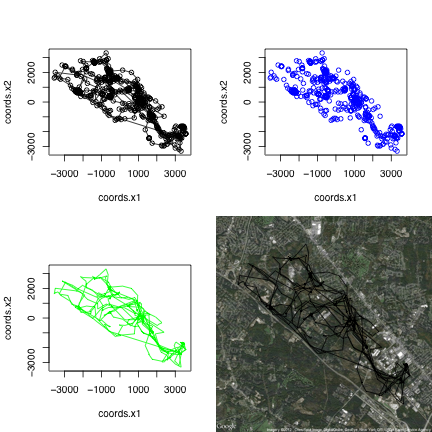
\includegraphics{move-fig1}
\end{center}
\caption{Plotting the UD (left) and adding the track as a line (center) or as points(right)}
\label{fig:two}
\end{figure}

To plot contour lines from the raster use the \fct{contour} function and set the percentage levels that you want to print. With \texttt{add=TRUE} you can add the contour to a previous plot (see Figure \ref{fig:three}). \\

\begin{figure}
\begin{center}
\begin{Schunk}
\begin{Sinput}
> plot(ricky_dbbmm, xlab="location_long", ylab="location_lat")
> contour(ricky_dbbmm, levels=c(.5, .95), col=c(6,2), add=TRUE, lwd=2)
\end{Sinput}
\end{Schunk}
\includegraphics{move-contour}
\end{center}
\caption{Plotting the 95\% and 50\% contour lines on top of the UD.}
\label{fig:three}
\end{figure}

\fct{raster}              : returns the information of the stored raster\\
\fct{outerProbability}    : calculates the probabilities of the UD at the border of the raster\\

\newpage

\section{Home Range Bootstrap using Minimum Convex Polygons}
The move package includes a method to calculate minimum convex polygons (MCP) using \fct{hrBootstrap}. A minimum convex polygon describes an area that is formed by the points of a track. It is called convex because no line that connects two points within this polygon crosses the border of the polygon. \\
We implemented the method to calculate MCPs from the adehabitatHR package (more information) using a bootstrap method. This means, that the area size of the MCP is calculated with an (exponential) increasing number of coordinates. Thus the MCP size is increasing as well until it reaches a plateau. \\
Because the function takes random coordinates to calculate the MCP every calculation is repeated by default 100 times. For every number of coordinates the quantiles are calculated and plotted in a line diagram. A black horizontal line indicates the real MCP size (calculated with all coordinates).

\begin{figure}
\begin{center}
\begin{Schunk}
\begin{Sinput}
> hrBootstrap(x=leroy, rep=100, unin='km', unout='km2')
\end{Sinput}
\end{Schunk}
\includegraphics{move-hrBootstrap}
\end{center}
\caption{The returned plot form the \fct{hrBootstrap} for a track with 100 repetitions.}
\label{fig:four}
\end{figure}



\end{document}
